\section{Experiments}
\label{sec:experiments}

% Our evaluation agenda for \method includes the 
Our experiments focus on the following research questions: (1) How does a single \method model perform in the zero-shot inference mode on unseen graphs and queries compared to the baselines? (2) Does \method retain the quality metrics like \emph{faithfullness} and identify easy answers reachable by traversal? (3) How does the multi-source propagation issue affect the performance?

\subsection{Setup and Datasets}

\textbf{Datasets.} 
We employ 23 different \clqa datasets each with 14 standard query types and its own underlying KG with different sets of entities and relations. Following Section~\ref{sec:prelim}, we categorize the datasets into three groups (more statistics of the datasets and queries are provided in Appendix~\ref{app:datasets}):
\begin{itemize}[leftmargin=*]
    \item \emph{Transductive} (3 datasets) where training and inference graphs are the same $(\gtrain = \ginf)$ and test queries cover the same set of entities and relations: FB15k237, NELL995 and FB15k all from \citet{betae} with at most 100 answers per query.
    \item \emph{Inductive entity} $(e)$ (9 datasets) from \citet{galkin2022} where inference graphs extend training graphs $(\gtrain \subset \ginf)$ being up to 550\% larger in the number of entities. The set of relations is fixed in each training graph and does not change at inference making the setup inductive with respect to the entities. Training queries might have more true answers in the extended inference graph.
    \item \emph{Inductive entity and relation} $(e,r)$ (11 datasets): we sampled a novel suite of WikiTopics-QA datasets due to the absence of standard benchmarks evaluating the hardest inductive setup where inference graphs have both new entities and relations $(\gtrain \neq \ginf)$. The source graphs were adopted from the WikiTopics datasets~\citep{isdea}, we follow the \emph{BetaE setting} when sampling 14 query types with at most 100 answers. More details on the dataset creation procedure are in Appendix~\ref{app:datasets}. 
\end{itemize} 

\textbf{Implementation and Training.}
\method was trained on one FB15k237 dataset with complex queries for 10,000 steps with batch size of 32 on 4 RTX 3090 GPUs for 2 hours (8 GPU-hours in total). 
We initialize the model weights with an available checkpoint of \ultra reported in \citet{ultra}. 
Following the standard setup in the literature, we train the model on 10 query types and evaluate on all 14 patterns.
We employ \emph{product t-norm} and \emph{t-conorm} as non-parametric fuzzy logic operators to implement conjunction $(\wedge)$ and disjunction $(\lor)$, respectively, and use a simple $1-x$ negation.
For the ablation study, \methodlp uses the same frozen checkpoint (pre-trained on simple \emph{1p} link prediction) with scores thresholding to alleviate the multi-source propagation issue (\Cref{subsec:ultra_proj}).
More details on all hyperparameters are available in Appendix~\ref{app:hyperparams}.



\textbf{Evaluation Protocol.}
As we train an \method model only on one FB15k237 dataset and run zero-shot inference on other 22 graphs, the inference mode on those is \emph{inductive} $(e,r)$ since their entity and relation vocabularies are all different from the training set.

As common in the literature~\citep{betae,ren2023ngdb}, the answer set of each query is split into \emph{easy} and \emph{hard} answers. 
Easy answers are reachable by graph traversal and do not require inferring missing links whereas hard answers are those that involve at least one edge to be predicted at inference.
In the rank-based evaluation, we only consider ranks of \emph{hard} answers and filter out easy ones and report filtered Mean Reciprocal Rank (MRR) and Hits@10 as main performance metrics.

Other qualitative metrics include: (1) \emph{faithfullness}~\citep{emql}, \ie, the ability to recover \emph{easy} answers reachable by graph traversal. 
Here, we follow the setup in \citet{galkin2022} and measure the performance of training queries on larger inference graphs where the same queries might have new true answers;
(2) the ROC AUC score to estimate whether a model ranks easy answers higher than hard answers -- we compute ROC AUC over \emph{unfiltered} scores of easy answers as positive labels and hard answers as negative.
(3) Mean Absolute Percentage Error (MAPE)~\citep{gnn_qe} between the number of answers extracted from model's predictions and the number of ground truth answers (easy and hard combined) to estimate whether \clqa models can predict the cardinality of the answer set.


\textbf{Baselines.}
In transductive and inductive $(e)$ datasets, we compare a single \method model with the best reported models trained end-to-end on each graph (denoted as \emph{Best baseline} in the experiments): QTO~\citep{qto} for 3 transductive datasets (FB15k237, FB15k, and NELL995) and GNN-QE~\citep{galkin2022} for 9 inductive $(e)$ datasets.
While a single \method model has 177k parameters, the baselines are several orders of magnitude larger with a parameters count depending on the number of entities and relations, \eg, a QTO model on FB15k237 has 30M parameters due to having 2000$d$ entity and relation embeddings, and GNN-QE on a reference FB 175\% inductive $(e)$ dataset has 2M parameters.
For a newly sampled suite of 11 inductive $(e, r)$ datasets, we compare against the edge-type heuristic baseline introduced in \citet{galkin2022}. 
The heuristic selects the candidate nodes with the same incoming relation as the last hop of the query. 
More details on the baselines are reported in Appendix~\ref{app:hyperparams}

\subsection{Main Experiment: Zero-shot Query Answering}

\begin{table*}[t]
\centering
\caption{Zero-shot inference results of \method and ablated \methodlp on 23 datasets compared to the best reported baselines. \method was trained on one transductive FB15k237 dataset, \methodlp was only pre-trained on KG completion and uses scores thresholding. The \emph{no thrs.} version does not use any thresholding of intermediate scores (\Cref{subsec:ultra_proj}). The best baselines are trainable on each transductive and inductive $(e)$ dataset, and the non-parametric heuristic baseline on inductive $(e,r)$ datasets. }
%\scriptsize
\begin{adjustbox}{width=\textwidth}
\begin{tabular}{lrrrrrrrrrrrrrrrrr}\toprule
\multirow{3}{*}{Model} &\multicolumn{4}{c}{\textbf{Inductive} $(e,r)$ (11 datasets)} &\multicolumn{4}{c}{\textbf{Inductive} $(e)$ (9 datasets)} &\multicolumn{4}{c}{\textbf{Transductive} (3 datasets)} &\multicolumn{4}{c}{\textbf{Total Average} (23 datasets)} \\\cmidrule(l){2-5} \cmidrule(l){6-9} \cmidrule(l){10-13} \cmidrule(l){14-17}
&\multicolumn{2}{c}{EPFO avg} &\multicolumn{2}{c}{neg avg} &\multicolumn{2}{c}{EPFO avg} &\multicolumn{2}{c}{neg avg} &\multicolumn{2}{c}{EPFO avg} &\multicolumn{2}{c}{neg avg} &\multicolumn{2}{c}{EPFO avg} &\multicolumn{2}{c}{neg avg} \\\cmidrule(l){2-3} \cmidrule(l){4-5} \cmidrule(l){6-7} \cmidrule(l){8-9} \cmidrule(l){10-11} \cmidrule(l){12-13} \cmidrule(l){14-15} \cmidrule(l){16-17}
&\bf{MRR} &\bf{H@10} &\bf{MRR} &\bf{H@10} &\bf{MRR} &\bf{H@10} &\bf{MRR} &\bf{H@10} &\bf{MRR} &\bf{H@10} &\bf{MRR} &\bf{H@10} &\bf{MRR} &\bf{H@10} &\bf{MRR} &\bf{H@10} \\\midrule
Best baseline &0.014 &0.029 &0.004 &0.007 &\bf{0.328} &\textbf{0.469} &\bf{0.176} &\bf{0.297} &\bf{0.468} &\bf{0.603} &\bf{0.259} &\bf{0.409} &0.196 &0.276 &0.105 &0.173 \\ \midrule
\textsc{UltraQuery} 0-shot &\bf{0.280} &0.380 &\bf{0.193} &\bf{0.288} &0.312 &\bf{0.467} &0.139 &0.262 &0.411 &0.517 &0.240 &0.352 &\bf{0.309} &\bf{0.432} &\bf{0.178} &\bf{0.286} \\
\textsc{UltraQuery LP} 0-shot &0.268 &\bf{0.409} &0.104 &0.181 &0.277 &0.441 &0.098 &0.191 &0.322 &0.476 &0.150 &0.263 &0.279 &0.430 &0.107 &0.195 \\
\textsc{UltraQuery LP} no thrs. &0.227 &0.331 &0.080 &0.138 &0.246 &0.390 &0.085 &0.167 &0.281 &0.417 &0.127 &0.223 &0.242 &0.367 &0.088 &0.161 \\
\bottomrule
\end{tabular}
\end{adjustbox}
\label{tab:maintab1}
\vskip -0.1 in
\end{table*}
\begin{figure*}[t]
    \centering
    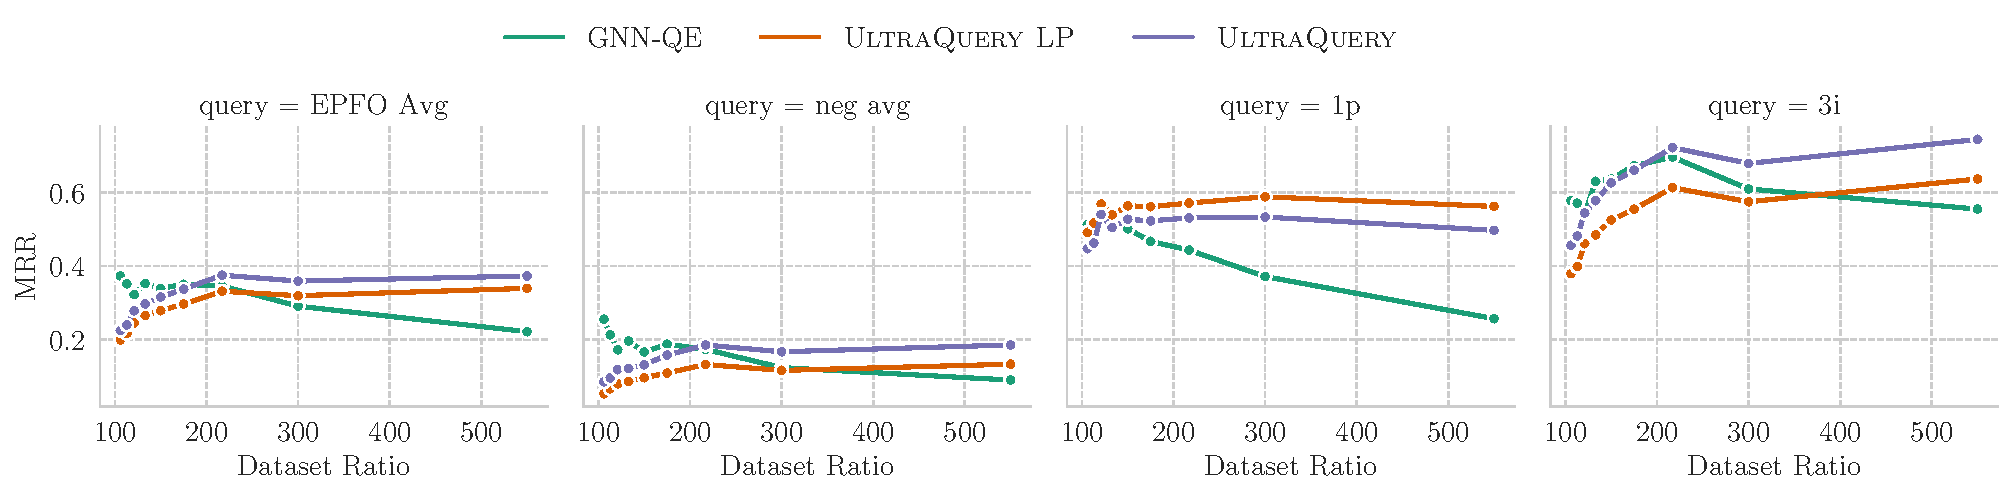
\includegraphics[width=\linewidth]{figs/newres_pyg.pdf}
    \vskip -0.1 in
    \caption{Mitigation of the multi-source message passing issue (Section~\ref{sec:method}) with \method: while \methodlp (pre-trained only on 1p link prediction) does reach higher 1p query performance (center right), it underperforms on negation queries (center left). \method adapts to the multi-source message passing scheme and trades a fraction of 1p query performance for better averaged EPFO, \eg, on the \emph{3i} query (right), and negation queries performance. More results are in Appendix~\ref{app:more_results}.}
    \label{fig:abl_multisource}
    \vskip -0.1 in
\end{figure*}

In the main experiment, we measure the zero-shot query answering performance of \method trained on a fraction of complex queries of one FB15k237 dataset. 
Figure~\ref{fig:main_fig1} and Table~\ref{tab:maintab1} illustrate the comparison with the best available baselines and ablated \methodlp model on 23 datasets split into three categories (transductive, inductive $(e)$, and inductive $(e,r)$). 
For each dataset, we measure the average MRR on 9 EPFO queries with projection, intersection, and union operators, and 5 negation queries with the negation operator, respectively.

Averaged across 23 datasets, \method outperforms available baselines by relative 50\% in terms of MRR and Hits@10 on EPFO and 70\% on negation queries (\eg, 0.31 vs 0.20 MRR on EPFO queries and 0.178 vs 0.105 on negation queries). 
The largest gains are achieved on the hardest inductive $(e,r)$ datasets where the heuristic baseline is not able to cope with the task. 
On inductive $(e)$ datasets, \method outperforms the trainable SOTA GNN-QE model on larger inductive inference graphs and performs competitively on smaller inductive versions. 
On transductive benchmarks, \method lags behind the SOTA QTO model which is expected and can be attributed to the sheer model size difference (177k of \method vs 30M of QTO) and the computationally expensive brute-force approach of QTO that materializes the whole $(\gV \times \gV \times \gR)$ 3D tensor of scores of all possible triples. 
Pre-computing such tensors on three datasets takes considerable space and time, \eg, 8 hours for FB15k with heavy sparsification settings to fit onto a 24 GB GPU.
%Besides, the FB15k dataset is known for years to have leakages~\citep{fb15k237} from inverse edges that large embedding models memorize and exploit. 
Still, \method outperforms a much larger QTO model on the FB15k dataset on both EPFO and negation queries.
The graph behind the NELL995 dataset is a collection of disconnected components which is disadvantageous for GNNs.

We note a decent performance of \methodlp trained only on simple \emph{1p} link prediction and imbued with score thresholding to alleviate the multi-source message passing issue described in Section~\ref{subsec:ultra_proj}.
Having a deeper look at other qualitative metrics in the following section, we reveal more sites where the issue incurs negative effects.


\subsection{Analysis}


\begin{figure*}[t]
    \centering
    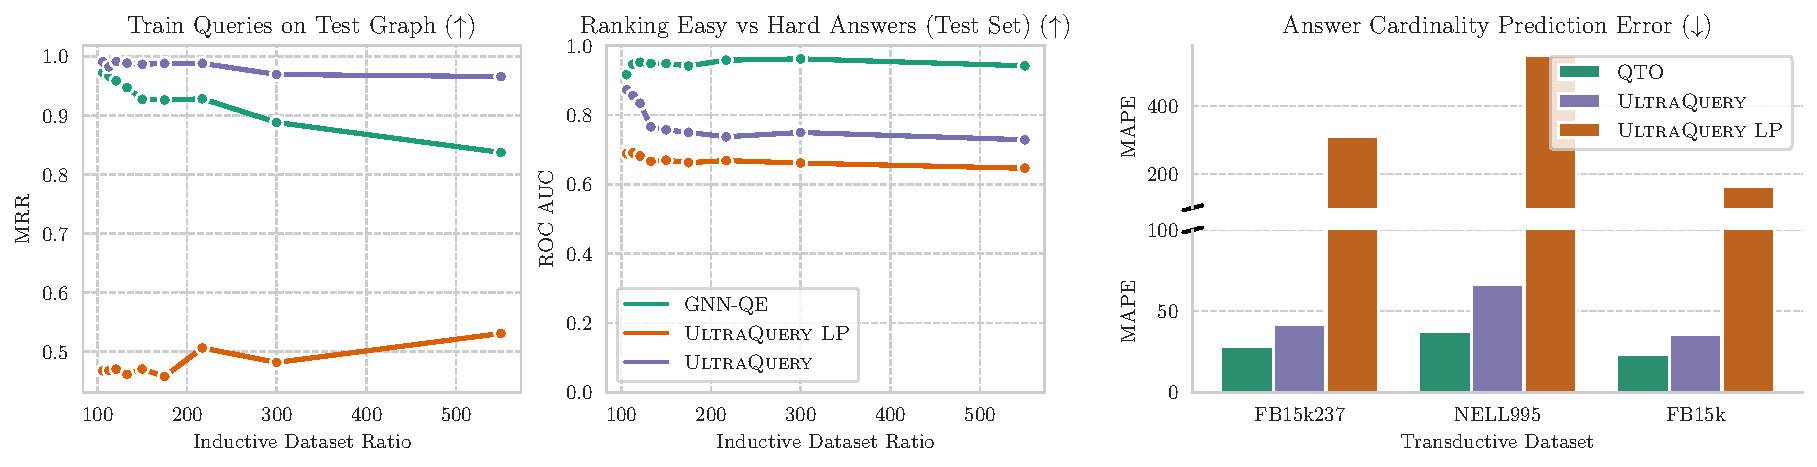
\includegraphics[width=\linewidth]{figs/qual_analysis_pyg.pdf}
    \vskip -0.1 in
    \caption{Qualitative analysis on 9 inductive $(e)$ and 3 transductive datasets averaged across all 14 query types. \textbf{Faithfullness, MRR (left):} \method successfully finds easy answers in larger inference graphs and outperforms trained GNN-QE baselines. \textbf{Ranking of easy vs hard answers, ROC AUC (center):} zero-shot inference methods slightly lag behind trainable GNN-QE due to assigning higher scores to hard answers. \textbf{Cardinality Prediction, MAPE (right):} \method is comparable to a much larger trainable baseline QTO. In all cases, \methodlp is significantly inferior to the main model. }
    \label{fig:abl_quality}
    \vskip -0.2 in
\end{figure*}

Here, we study four aspects of model performance: the effect of the multi-source message passing issue mentioned in Section~\ref{subsec:ultra_proj}, the ability to recover answers achievable by edge traversal (\emph{faithfullness}), the ability to rank easy answers higher than hard answers, and the ability to estimate the cardinality of the answer set.

\textbf{The multi-source message passing effect.}
%\zz{Maybe it's better to add results of \methodlp without thresholding.}
The pre-trained \ultra checkpoint used in \methodlp is tailored for singe-source message passing and struggles in the \clqa setup on later hops with several initialized nodes (\autoref{tab:maintab1}). 
Training \method on complex queries alleviates this issue as shown in \autoref{fig:abl_multisource}, \ie, while \emph{1p} performance of \methodlp is higher, the overall performance on EPFO and negative queries is lacking. 
In contrast, \method trades a fraction of \emph{1p} single-source performance to a much better performance on negative queries (about $2\times$ improvement) and better performance on many EPFO queries, for example, on \emph{3i} queries. 
Besides that, we note that the zero-shot performance of both \method models does not deteriorate from the increased size of the inference graph compared to the baseline GNN-QE.

\textbf{Recovering easy answers on any graph.}
\emph{Faithfullness}~\citep{emql} is the ability of a \clqa model to return \emph{easy} query answers, \ie, the answers reachable by edge traversal in the graph without predicting missing edges.
While faithfullness is a common problem for many \clqa models, \autoref{fig:abl_quality} demonstrates that \method almost perfectly recovers easy answers on any graph size even in the zero-shot inference regime in contrast to the best baseline.
Simple score thresholding does not help \methodlp to deal with complex queries as all easy intermediate nodes have high scores above the threshold and the multi-source is more pronounced. 

\textbf{Ranking easy and hard answers.}
A reasonable \clqa model is likely to score easy answers higher than hard ones that require inferring missing links~\citep{galkin2022}.
Measuring that with ROC AUC  (\autoref{fig:abl_quality}), \method is behind the baseline due to less pronounced decision boundaries (overlapping distributions of scores) between easy and hard answers' scores. 
Still, due to scores filtering when computing ranking metrics, this fact does not have a direct negative impact on the overall performance.

\textbf{Estimating the answer set cardinality.}
Neural-symbolic models like GNN-QE and QTO have the advantage of estimating the cardinality of the answer set based on the final scores without additional supervision. 
As shown in \autoref{fig:abl_quality}, \method is comparable to the larger and trainable QTO baseline on FB15k237 (on which the model was trained) as well as on other datasets in the zero-shot inference regime. 
Since cardinality estimation is based on score thresholding, \methodlp is susceptible to the multi-source propagation issue with many nodes having a high score and is not able to deliver a comparable performance.


\begin{wrapfigure}{R}{0.5\textwidth}
\begin{minipage}{0.5\textwidth}
\vspace{-3em}
    \centering
    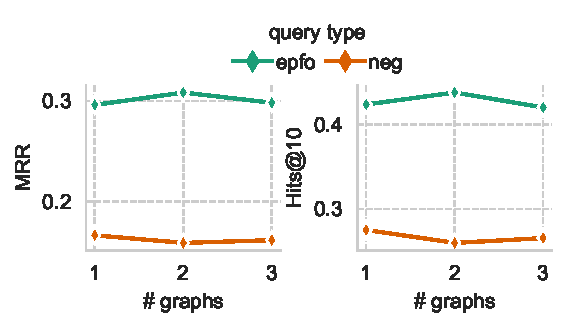
\includegraphics[width=1.0\linewidth]{figs/ultraquery_num_graphs.pdf}
    \caption{Average MRR (left) and Hits@10 (right) of 9 inductive $(e)$ and 11 inductive $(e,r)$ \clqa datasets for EPFO and negation queries depending on the number of graphs in the training mix.}
    \label{fig:num_graphs1}
    \vspace{-1em}
\end{minipage}
\end{wrapfigure}


\textbf{Varying the number of graphs in training.}
\autoref{fig:num_graphs1} and \autoref{tab:rebuttal2} report the inductive inference \clqa performance depending on the number of KGs in the training mixture. 
The original \method was trained on queries from the FB15k237. 
In order to maintain the zero-shot inductive inference setup on 11 inductive $(e,r)$ and 9 inductive $(e)$ datasets, we trained new model versions on the rest of BetaE datasets, that is, \method \textsc{2G} combines FB15k237 and NELL995 queries (trained for 20k steps), \method \textsc{3G} combines FB15k273, NELL995, and FB15k queries (trained for 30k steps). %The training parameters are the same as in the Appendix B and Table 9 from the original paper except that the \method \textsc{2G} was trained for 20k steps and \method \textsc{3G} was trained on 30k steps (reported in Table~\ref{tab:rebuttal1}).
The most noticeable improvement of \textsc{2G} and \textsc{3G} versions is the increased MRR and Hits@10 on EPFO queries (9 query types) on 11 inductive $(e,r)$  datasets yielding about 10\% gains.
On 9 inductive $(e)$ datasets the performance is either on par with the \textsc{1G} version or a bit lower. 
Averaged across 20 datasets, the \textsc{2G} version exhibits the best EPFO performance at the cost of slightly reduced negation query performance.




\begin{table}[t]
\centering
\caption{Zero-shot inference results (on 20 inductive datasets) of \method trained on 1, 2, and 3 datasets, respectively. The biggest gains of the 2G model are \textbf{in bold}.}
\label{tab:rebuttal2}
%\scriptsize
\begin{adjustbox}{max width=\textwidth}
\begin{tabular}{lrrrrrrrrrrrrr}\toprule
\multirow{3}{*}{Model} &\multicolumn{4}{c}{\textbf{Inductive} $(e,r)$ (11 datasets)} &\multicolumn{4}{c}{\textbf{Inductive} $(e)$ (9 datasets)} &\multicolumn{4}{c}{\textbf{Total Average} (20 datasets)} \\\cmidrule{2-13}
&\multicolumn{2}{c}{EPFO avg} &\multicolumn{2}{c}{neg avg} &\multicolumn{2}{c}{EPFO avg} &\multicolumn{2}{c}{neg avg} &\multicolumn{2}{c}{EPFO avg} &\multicolumn{2}{c}{neg avg} \\\cmidrule{2-13}
&\bf{MRR} & \bf{H@10} & \bf{MRR} &\bf{H@10} &\bf{MRR} &\bf{H@10} &\bf{MRR} &\bf{H@10} &\bf{MRR} &\bf{H@10} &\bf{MRR} &\bf{H@10} \\\midrule
\method 1G &0.280 &0.380 &0.193 &0.288 &0.312 &0.467 &0.139 &0.262 &0.296 &0.423 &0.166 &0.275 \\
\method 2G & \bf{0.310} & \bf{0.413} &0.187 &0.275 &0.307 &0.463 &0.130 &0.244 &0.308 &0.438 &0.158 &0.260 \\
\method 3G &0.304 &0.402 &0.195 &0.292 &0.292 &0.438 &0.127 &0.239 &0.298 &0.420 &0.161 &0.265 \\
\bottomrule
\end{tabular}
\end{adjustbox}
\vspace{-1em}
\end{table}